\section{Fibrations and cofibrations}
\subsection{Comparing fibers over different points}
Let $p:E\to B$ be a fibration.
Above, we saw that this implies that paths in $B$ ``lift'' to paths in $E$.
Let us consider a path $\omega:I\to B$ with $\omega(0) = a$ and $\omega(1) = b$.
Denote by $F_a$ the fiber over $a$. 
If the world plays fairly, the path lifting property of fibrations should beget a (unique\footnote{At least up to homotopy.})
map $F_a\to F_b$.
The goal of this subsection is to construct such a map.

Consider the diagram:
\begin{equation*}
    \xymatrix{
	F_a\ar[d]_{\mathrm{in}_0}\ar[rr] & & E\ar[d]^p\\
	I\times F_a\ar@{-->}[urr]^{h}\ar[r]_{\mathrm{pr}_1} & I\ar[r]_{\omega} & B.
    }
\end{equation*}
This commutes since $\omega(0) = a$.
Utilizing the homotopy lifting property, there is a dotted arrow that makes the entire diagram commute.
If $x\in F_a$, the image $h(1,x)$ is in $F_b$, and $h(0,x) = x$.
This supplies us with a map $f:F_a\to F_b$, given by $f(x) = h(1,x)$.

We're now faced with a natural question: is $f$ unique up to homotopy?
Namely: if we have two homotopic paths $\omega_0,\omega_1$ with $\omega_0(0) = \omega_1(0) = a$,
and $\omega_0(1) = \omega_1(1) = b$, along with a given homotopy $g:I\times I\to B$ between $\omega_0$ and $\omega_1$,
such that $f_0,f_1:F_a \to F_b$ are the associated maps (defined by $h_0(1,x)$ and $h_1(1,x)$),
respectively, are $f_0$ and $f_1$ homotopic?

We have a diagram of the form:
\begin{equation*}
    \xymatrix{
	((\partial I\times I)\cup (I\times \{0\}))\times F_a\ar[d]_{\mathrm{in}_0}\ar[rr] & & E\ar[d]^p\\
	I\times I\times F_a\ar[r]_{\mathrm{pr}_1}\ar@{-->}[urr] & I\times I\ar[r]_g & B
    }
\end{equation*}
To get a homotopy between $f_0$ and $f_1$, we need the dotted arrow to exist.

% Add a picture, maybe?
%
%Think of the space $(\partial I\times I)\cup (I\times 0)$ as follows:
%\begin{equation*}
%\begin{tikzpicture}
%    \draw (2,2) -- (0,2) -- (0,0) -- (2,0);
%    \node [above] at (1,2) {$h_1$};
%    \node [below] at (1,0) {$h_0$};
%    \node [left] at (0,1) {$in_0$};
%\end{tikzpicture}
%\end{equation*}
%and $I\times I$ looks like:
%\begin{equation*}
%    \begin{tikzpicture}
%	\draw (0,0) -- (0,2) -- (2,2) -- (2,0) -- (0,0);
%	\draw[fill] (2,2) circle [radius=0.05];
%	\draw[fill] (2,0) circle [radius=0.05];
%	\node [left] at (0,1) {$a$};
%	\node [above] at (1,2) {$\omega_1$};
%	\node [below] at (1,0) {$\omega_0$};
%	\node [right] at (2,1) {$b$};
%	\node [above right] at (2,2) {$f_1$};
%	\node [below right] at (2,0) {$f_0$};
%    \end{tikzpicture}
%\end{equation*}
%
%Does the dotted map exist? Clearly this is crying out for us to use the homotopy lifting property. But what should our space $W$ be? Well the following pair:
%\begin{equation*}
%    \begin{tikzpicture}
%	\draw (2,2) -- (0,2) -- (0,0) -- (2,0);
%    \end{tikzpicture}\subseteq
%    \begin{tikzpicture}
%	\draw (0,0) -- (0,2) -- (2,2) -- (2,0) -- (0,0);
%    \end{tikzpicture}
%\end{equation*}
%is homotopy equivalent to $(0\subseteq I)\times I$. Hence in our diagram we now have:

It's an easy exercise to recognize that our diagram is equivalent to the following.
\begin{equation*}
    \xymatrix{
	I\times F_a\ar[rr]^{\simeq} & & ((\partial I\times I)\cup (I\times 0))\times F_a\ar[d]_{\mathrm{in}_0}\ar[rr] & & E\ar[d]^p\\
	I\times I\times F_a\ar[rr]_{\simeq} & & I\times I\times F_a\ar[r]_{\mathrm{pr}_1}\ar@{-->}[urr] & I\times I\ar[r]_g & B
    }
\end{equation*}
Letting $W=I\times F_a$ in the definition of a fibration (Definition \ref{fibration}) thus gives us the desired lift,
i.e., a homotopy $f_0\simeq f_1$.

We can express the uniqueness (up to homotopy) of lifts of homotopic paths in a functorial fashion.
To do so, we must introduce the fundamental groupoid of a space.
\begin{definition}
    Let $X$ be a topological space.
    The \emph{fundamental groupoid} $\Pi_1(X)$ of $X$ is a category (in fact, groupoid),
    whose objects are the points of $X$, and maps are homotopy classes of paths in $X$.
    The composition of compatible paths $\sigma$ and $\omega$ is defined by:
    \begin{equation*}
	(\sigma\cdot\omega)(t) = \begin{cases}
	    \omega(2t) & 0\leq t\leq 1/2\\
	    \sigma(2t - 1) & 1/2\leq t\leq 1.
	\end{cases}
    \end{equation*}
\end{definition}
The results of the previous sections can be succintly summarized in the following neat statement.
\begin{prop}
    Any fibration $p:E\to B$ gives a functor $\Pi_1(B)\to \Top$.
\end{prop}
This is the beginning of a beautiful story involving fibrations.
(The interested reader should look up ``Grothendieck construction''.)

\subsection{Cofibrations}
Let $i:A\to X$ be a map of spaces.
If $Y$ is another topological space, when is the induced map $Y^X\to Y^A$ a fibration?
This is asking for the map $i$ to be ``dual'' to a fibration.

By the definition of a fibration, we want a lifting:
\begin{equation*}
    \xymatrix{
	W\ar[r]\ar[d]_{\mathrm{in}_0} & Y^X\ar[d]\\
	I\times W\ar@{-->}[ur]\ar[r] & Y^A.
    }
\end{equation*}
Adjointing over, we get:
\begin{equation*}
    \xymatrix{
	A\times W\ar[r]^{i\times 1}\ar[d]_{1\times \mathrm{in}_0} & X\times W\ar[d]\ar[ddr]& \\
	A\times W\times I \ar[r]\ar[drr] & X\times I\times W\ar@{-->}[dr] & \\
	& & Y.
    }
\end{equation*}
Again adjointing over, this diagram transforms to:
\begin{equation*}
    \xymatrix{
	A\ar[r]\ar[d] & X\ar[d]\ar[ddr] & \\
	A\times I\ar[r]\ar[drr] & X\times I\ar@{-->}[dr] & \\
	& & Y^W.
    }
\end{equation*}
This discussion motivates the following definition of a ``cofibration'':
as mentioned above, this is ``dual'' to the notion of fibration.

\begin{definition}\label{cofibration}
    A map $i:A\to X$ of spaces is said to be a \emph{cofibration} if it satisfies the
    \emph{homotopy extension property} (sometimes abbreviated as ``HEP''):
    for any space $Y$, there is a dotted map in the following diagram that makes it commute:
    \begin{equation*}
    \xymatrix{
	A\ar[r]\ar[d] & X\ar[d]\ar[ddr] & \\
	A\times I\ar[r]\ar[drr] & X\times I\ar@{-->}[dr] & \\
	& & Y.
    }
    \end{equation*}
\end{definition}

Again, using the definition of a pushout, the universal example of such a space $Y$ is the pushout $X\cup_A (A\times I)$.
Equivalently, we are therefore asking for the existence of a dotted arrow in the following diagram.
\begin{equation*}
    \xymatrix{
	X\cup_A (A\times I)\ar[r]\ar[dr] & X\times I\ar@{-->}[d]\\
	& Z,
    }
\end{equation*}
for any $Z$.
Using the universal property of a pushout, this is equivalent to the existence of a dotted arrow in the following diagram.
\begin{equation*}
    \xymatrix{
	X\cup_A (A\times I)\ar[r]\ar[dr] & X\times I\ar@{-->}[d]\\
	& X\cup_A(A\times I)\ar[d]\\
	& Z,
    }
\end{equation*}
which is, in turn, equivalent to asking $X\cup_A (A\times I)$ to be a retract of $X\times I$.

\begin{example}
    $S^{n-1}\hookrightarrow D^n$ is a cofibration.
    \todo{Properly draw out this figure!}
    \begin{figure}[H]
	\centering
	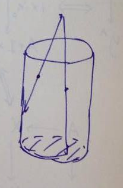
\includegraphics[scale=0.75]{assets/retract-cofibration}
	\caption{Drawing by John Ni.}
    \end{figure}
    In particular, setting $n=1$ in this example, $\{0,1\}\hookrightarrow I$ is a cofibration.
\end{example}

Here are some properties of the class of cofibrations of CGWH spaces.
\begin{itemize}
    \item It's closed under cobase change: if $A\to X$ is a cofibration, and $A\to B$ is any map,
	the pushout $B\to X\cup_A B$ is also cofibration. (Exercise!)
    \item It's closed under finite products. (This is surprising.)
    \item It's closed under composition. (Exercise!)
    \item Any cofibration is a closed inclusion\footnote{Note that the dual statement for
	fibrations would state:	any fibration $p:E\to B$ is a quotient map.
	This is definitely not true: fibrations do not have to be surjective!
	For instance, the trivial map $\emptyset\to B$ is a fibration.
	(Fibrations are surjective on path components though, because of path lifting.)}.
	\todo{This is not obvious; should we include a proof?}
\end{itemize}
